\documentclass{standalone}
\usepackage{tikz}
\usetikzlibrary{calc}
\usetikzlibrary{decorations.pathreplacing,calligraphy}
\usepackage{pgfplots}
\usetikzlibrary{intersections, pgfplots.fillbetween}
\usetikzlibrary{snakes}
\usepackage{xcolor}

\begin{document}

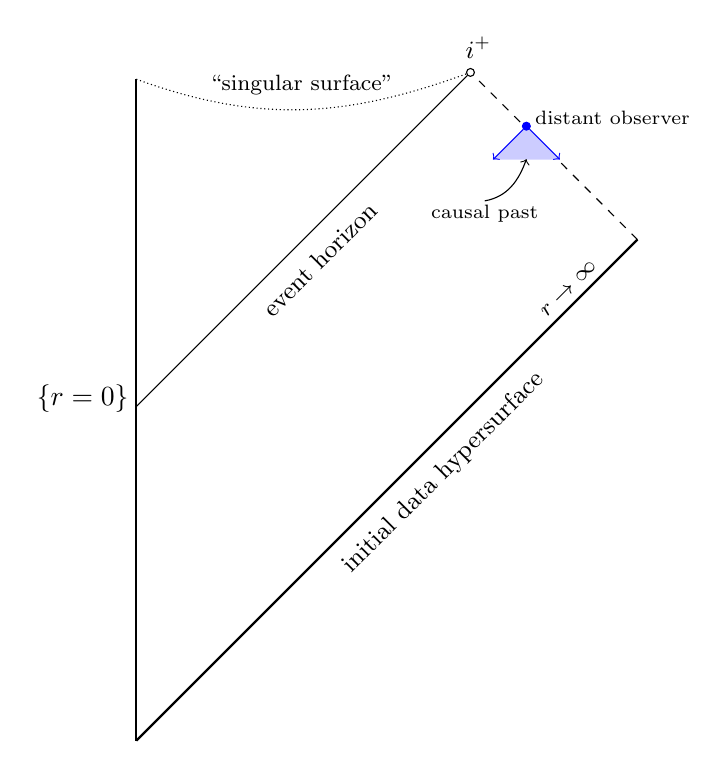
\begin{tikzpicture}[scale=1.5]


\coordinate (n1) at (0,0);
\coordinate (n2) at (45:6);
\draw[thick] (n1) -- (n2);
\coordinate (n3) at ($(n2) + (135:2) $);
\node[circle, inner sep = 0, minimum size = .1cm, label = {[xshift=1mm]above:\small{$i^+$}}, draw] (node1) at (n3) {};
\draw[dashed] (n2) -- (node1);

\coordinate (n4) at ($(n1) + (0,5.6) $);
\draw[thick] (n1) -- (n4);

\draw[densely dotted] (n4) to[out = -20, in = 200] (node1);


\node[label = left:{$\{r=0\}$}] at ($(0,2.9) + (.1,0)$) {};

\draw[] (node1) --+ (-135:4);
\coordinate (n5) at ($(n3) + (-135:2)$);
\node[label = {[rotate=45]below:\small{ event horizon}}] at (n5) {};

\coordinate (n6) at ($(n4) + (1.4,0) + (0,-.3) $);
\node[label = above:\footnotesize{``singular surface''}] at (n6) {};

\coordinate (n7) at (45:3) ;
\node[label = {[rotate = 45]below:\small{initial data hypersurface}}] at ($(n7) +(45:.5)$){};


\coordinate (n95) at ($(0,1.9) + (45:4.67) $ );
\coordinate (n10) at ($(n95) + (-45:.4) $);
\coordinate (n11) at ($(n95) + (-135:.4) $);
\fill[blue!20] ($(0,1.9) + (45:4.67) $ ) -- (n10) -- (n11);
\node[circle, blue, fill, draw, inner sep = 0, minimum size = .1cm, label = {[yshift = 1mm, xshift = -.7mm]right:\scriptsize{distant observer}}] (obs) at (n95) {};

\draw[->, blue] (obs) -- (n10) ;
\draw[->, blue] (obs) -- (n11) ;

\coordinate (n12) at ($(n95) + (0,-.28) $);
\coordinate (n13) at ($(n12) + (-135:.5) $ );

\draw[->] (n13) to[out=10, in = -110] (n12);

\node[label = {[yshift = 2mm]below:\scriptsize{causal past}}] at (n13) {};

\node[label = {[rotate = 45,yshift=-1mm]above:\footnotesize{ $ r\rightarrow \infty $ }}] at ($(n7) +(45:2.2)$) {};


\end{tikzpicture}


\end{document}